% !TEX root = /Users/zhuzhuangdi/Desktop/MSUCourses/MachineLearning847/17Project/17spr_wang_zhu_du/Middle/middle_report.tex
\section{Project Milestones} 

\subsection{Completed Milestones} 
%
\subsubsection{Background Survey}
 For this initial step, we plan to search for related works to computational literary creation to gain the basic knowledge of Song Ci.
%
We are interested in the following questions: what is the criterion of a good Song Ci? How to evaluate the correctness, fluency and style of poems generated?
%
Better understanding of related work and Song Ci composition rules will provide us with great help for the following work, especially algorithm testing and comparison. 
%
\subsubsection {Corpus Search and Analysis}
%

\nan{ describe corpus: size, content, etc.}
We collected corpus that are comprehensive on poem styles, and are precisely analyzed for content. 

\wei{ insert a  picture of word-frequency analysis.}
%
\subsubsection{ Implementation of a Vector Space Model }
Vector space models (VSMs) represent words in a continuous vector space where semantically similar words are mapped to nearby points.
%
We implemented this model to find the semantic relations between each Chinese character, so that given a few of keyword characters, such as 'spring' and 'beauty', we can generate poetries with coherent meanings using characters which are close to these keywords in the vector space.
%
%We use a predictive method to implement this  model based on the TensorFlow programming package \cite{tensorflow}.
%
We give a visualized result in Figure \ref{fig:VSM}. The figure is embeded with 100 Chinese characters in a 2-D space, which are randomly chosen from the most frequent 500 Chinese characters in the Song Ci corpus. The 2-D space corresponds to the first two dimensions in the vector space.
\begin{figure}[htbp]
	\centering
	\includegraphics[width=0.9\linewidth]{tsne.png}
	\caption{Vector Space Model}
	\label{fig:VSM}	
\end{figure} 
\subsubsection{ Implementation of a RNN + LSTM Model  }   
We implement a preliminary version of our model. It is a special kind of RNN with Long Short Term Memory units (LSTM), which can capture long-term dependencies.
%
The reasonale of applying LSTM to our model is that,  different from Tang poetry, Song Ci has more content  and is variant in styles.
%
We may lose the coherent meaning of the generated Song Ci without backtracking previous context.
%

%VSMs have a long, rich history in NLP, but all methods depend in some way or another on the Distributional Hypothesis, which states that words that appear in the same contexts share semantic meaning. The different approaches that leverage this principle can be divided into two categories: count-based methods (e.g. Latent Semantic Analysis), and predictive methods (e.g. neural probabilistic language models).
%Test cases will be generated with both poem generator under the same keywords and topics. Poems will be test on aspects of grammar, semantic correctness, style and content. Both computational evaluation and human evaluation are expected to be used in last part of our project.
%Third, implementation poem generator based on both algorithm of RNN and genetic algorithm would be the most important work in our project. So we will assign more time on this step. 
%
We present a prelimanry result in Figure \ref{fig:poetry}. 

 
\begin{figure}[htbp]
	\centering
	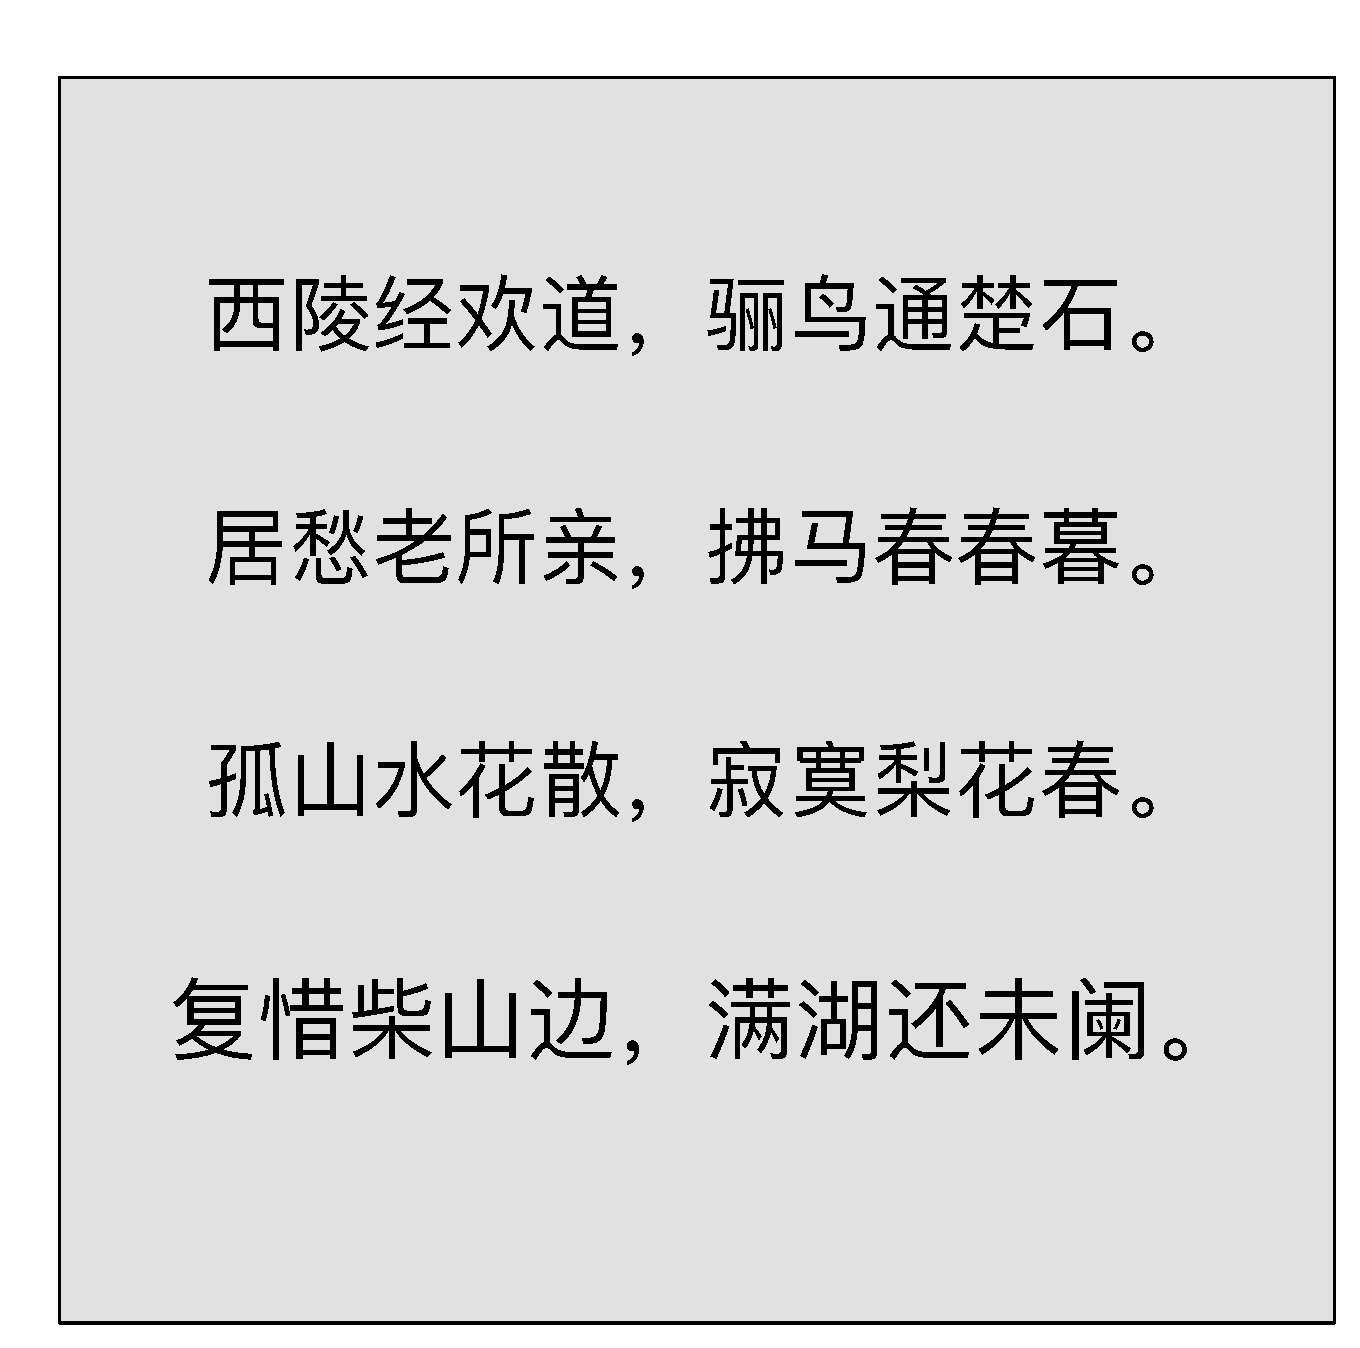
\includegraphics[width=0.8\linewidth]{poetry}
	\caption{A poetry generated using RNN+LSTM model}
	\label{fig:poetry}	
\end{figure} 


\subsection{Remaining Milestones}
%
\subsubsection{Implementation of Song Ci Generating Model }
\subsubsection{Model Testing and Comparison}
\subsubsection{Project Writing} 
